%---------------------------------------------------------%
%______//------             GAC             ------\\______%
%______||------         Chapitre 7          ------||______%
%______\\------      Graphes de Cayley      ------//______%
%---------------------------------------------------------%

\chapter{Graphes de Cayley (groupes comme espaces métriques)}
\label{sec:graphes-de-Cayley}

  Soit $G$ un groupe, $S \subset G$ une partie symétrique ($s \in S \Rightarrow s^{-1} \in S$) et $1 \notin
  S$.

  \begin{defi} \index{Graphe!de Cayley}
    Le \emph{graphe de Cayley}, noté $\Gamma(G, S)$ est le graphe dont l'ensemble des sommets est $G$ est
    l'ensemble des arêtes est $E = \{(x,y) | xy^{-1} \in S \iff \exists s \in S\ :\ y = xs\}$.

    Deux sommets sont \emph{voisins}, et on les notes $x \sim y$, si $y$ s'obtient à partir de $x$ par
    multiplication par un élément de $S$.
  \end{defi}

  \begin{exs}
    \begin{enumerate}
    \item Soit $G = \Z/6\Z$ et $S = \{x, x^{-1}\}$, pour $x = 1$ et $x^{-1} = 5$.

    \item Soit $G = \Z/6\Z$ et $S = \{2, -2\}$.

    \item Soit $G = \Z/6\Z$ et $S = \{3 = -3\}$.

    \item Soit $G = \Z/6\Z$ et $S = \{2, -2, 3 = -3\}$.

    \item Soit $G = \Z$ et $S = \{1, -1\}$.

    \item Soit $G = \Z^2$ et $S = \{(\pm 1, 0), (0, \pm 1)\}$.

    \item Soit $G = \F_2 = \F(a,b)$ le groupe libre avec 2 générateurs et soit $S = \{a^{\pm 1}, b^{\pm 1}\}$.
    \end{enumerate}
  \end{exs}

  \begin{propri}
    \begin{enumerate}
    \item $\Gamma(G,S)$ est $k$-régulier, où $k = |S|$ (c'est-à-dire tout sommet a $k$ voisins).
    \item $\Gamma(G,S)$ et connexe $\iff$ $S$ engendre $G$.
    \end{enumerate}
  \end{propri}

  \begin{defi} \index{Arbre}
    Un \emph{arbre} un graphe connexe sans chemins fermés.
  \end{defi}

  \begin{prop}
    Soit $G$ un groupe et $S \subseteq G$ un ensemble. Alors $G cong \F(S)$ (le groupe libre sur $S$) si et
    seulement si $\Gamma(G, S)$ est un arbre.
  \end{prop}


  \begin{defi}
    Soient $\Gamma_1 = (V_1, E_1)$ et $\Gamma_2 = (V_2, E_2)$ deux graphes. Un \emph{morphisme de graphe}
    \index{Morphisme!de graphe} est une application $\phi: \Gamma_1 \to \Gamma_2$, $\phi \big|_V : V_1 \to
    V_2$, $\phi \big|_E : E_1 \to E_2$ telle que $(\phi(v), \phi(v')) \in E_2 \iff (v, v') \in E_1$.

    Si $\phi$ est bijective et $\Gamma_1 = \Gamma_2$, $\phi$ s'appelle un \emph{automorphisme de graphe}.
    \index{Automorphisme!de graphe}

    L'ensemble de tous les automorphisme de $\Gamma$, noté $Aut(\Gamma)$ forme un groupe.
  \end{defi}


  \begin{theo}
    Soit $G$ un groupe dénombrable. Alors il y a un graphe connexe $X$ tel que $G \cong Aut(X)$.
  \end{theo}

  \begin{preuve}
    Soit $S = \{s_1, s_2, \ldots \}$ un ensemble dénombrable de générateurs, c'est-à-dire que $G = \langle S
    \rangle$. Soit $X_0 = \Gamma(G,S)$ le graphe de Cayley de $G$ par rapport à $S$. Il faut se convaincre que
    $G \not\cong Aut(X_0)$.

    Pour chaque $i \geq 1$, soit $T_i$ un arbre fini (qui correspond à $s_i$)
    \begin{center}
      Figure de $T_i$ ici.
    \end{center}
    Si $i \neq j$, on a que $T_i \not\cong T_j$, car on n'a pas le même nombre de sommets dans $T_i$ et
    $T_j$. On doit montrer que $Aut(T_i) = \{id\}$ (exercice). 

    Dans le graphe de Cayley $X_0$, on remplace chaque arête $s_i$ par $T_i$, par exemple
    \begin{center}
      Dessiner exemple ici
    \end{center}
    et on obtient un graphe $X$. On a ainsi une expansion de $X_0$ vers $X$ ainsi qu'une contraction de $X$
    vers $X_0$ (en remplaçant $T_i$ par $s_i$). On observe que chaque automorphisme $\phi: X \to X$ induit un
    automorphisme $\phi_0: X_0 \to X_0$. 
    \begin{enumerate}
    \item Si $\gamma \in Aut(X)$ fixe $x \in V(X)$ ($\gamma(x) = x$), alors $\gamma = id_X$. En effet, si $x
      \in V(X) \setminus V(X_0)$ et $\gamma(x) = x$, alors $x \in V(T_i) \setminus \{a_i, b_i\}$. Ainsi
      $\gamma(T_i) = T_i$. Supposons que $x \in V(X_0)$ et $\gamma(T_{x,j}) = T_{x,j}$ pour chaque $x \in
      T_{x,j}$. L'idée est que si on fixe un tel $x$, on est obligé de fixer l'arbre $T_{x,j}$ (car deux
      arbres différents ne sont pas isomorphes), ainsi on fixe tous les arbres, donc toutes les arêtes et
      ainsi on fixe $xs_i$ pour chaque $i$, et par le Lemme de Zorn (car c'est un arbre infini, donc on doit
      faire ce processus à l'infini), on fixe l'arbre. C'est-à-dire que $\gamma(X) = X$, donc $\gamma = id$.

    \item $Aut(X) \cong G$. Soit $\phi: G \to Aut(X)$, $g \mapsto \phi_g$ où $\phi_g : X \to X$ est une
      extension de $\phi_g^0: X_0 \to X_0$ et $\phi_g^0(v) = gv$ si $v \in V(X_0) = G$. Commençons par montrer
      que $\phi$ est injective. On a
      \begin{align*}
        \phi(g) = \phi(g') &\iff \phi_g(v) = \phi_{g'}(v)\\
        &\iff gv = g'v\\
        &\iff g = g'
      \end{align*}
      Montrons à présent que $\phi$ est surjective. Soit $\psi \in Aut(X)$ avec $\psi(v) = v'$ pour $v,v' \in
      X_0$, alors il existe $g \in G$ tel que $\phi_g(v) = v'$ (par exemple on prend $g = v'v^{-1}$). On a
      $\psi(v) = \phi_g(v)$, et ainsi $(\psi^{-1}\phi_g)(v) = v$ et par la première observation,
      $\psi^{-1}\phi_g = id$ et donc $\psi = \phi_g$. \qedhere
    \end{enumerate}
  \end{preuve}

  \begin{rem}
    Si on change l'ensemble $S$, les graphes de Cayley pour $G$ sont différents entre eux (c'est-à-dire qu'ils
    ne sont pas isomorphes, en général). Mais ils sont \emph{quasi-isométriques} \index{Graphe!quasi-isométrique}
  \end{rem}


  À présent, on supposera toujours que $S$ engendre $G$ (sinon le graphe n'est pas connexe, et on n'a pas des
  bonnes propriétés).

  \begin{defi} \index{Longueur d'un mot $g$}
    Soit $g \in G$. La \emph{longueur} des mots de $g$ est la distance de $g$ à $\epsilon$ dans $\Gamma(G,S)$.
      \[|g|_S := \min\{n \in \N\ |\ g = s_1\cdots s_n,\ s_i \in S\}.\]

    Pour $g \in G$, la \emph{distance} de $x$ a $y$ \index{distance entre deux mots} est celle dans
    $\Gamma(G,S)$, notée $d_S(x,y) = |x^{-1}y|_S$.
  \end{defi}

  \begin{obss}
    \begin{enumerate}
    \item $d_S: G \times G \to \N$ est une distance sur $G$, invariante par l'action à gauche de $G$, $d_S(gx,
      gy) = d_S(x,y)$.

    \item Cette distance dépend du choix d'un système de générateurs $S$. Mais on va voir qu'en regardant le
      groupe \og de loin\fg, plusieurs propriétés importantes ne dépendent pas de $S$ (Gromov, $\sim 1980$).
    \end{enumerate}
  \end{obss}

  \begin{ex}
    Considérons $G = \Z$ et $S = \{\pm 1\}$. Le graphe de Cayley est simplement une droite infinie à gauche et
    à droite. Si à présent on considère $S' = \{\pm 2, \pm 3\}$, le graphe de Cayley devient 
    \begin{center}
    
            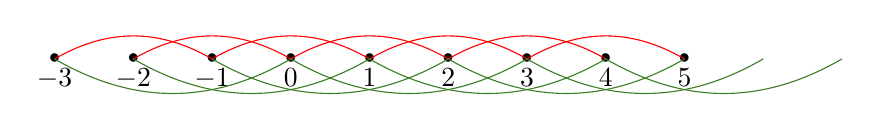
\begin{tikzpicture}
              \foreach \k in {-3,-2,...,5} { \draw (\k, 0) node[scale=0.8]{$\bullet$} node[below]{$\k$}; }
              \foreach \k in {-3, -2, ..., 3}{ \draw[color = red] (\k, 0) to[bend left] ({\k+2}, 0); }
              \foreach \k in {-3, -2, ..., 4}{ \draw[color = OliveGreen] (\k, 0) to[bend right] ({\k+3}, 0); }
            \end{tikzpicture}

          \end{center}
  \end{ex}

 
  

  

  




%%% Local Variables:
%%% mode: latex
%%% TeX-master: "../GAC_cours.tex" 
%%% End: